% =============================================================================
% Lecture 03: Generalized Additive Models (GAMs)
% ECON 8310: Business Forecasting
% University of Nebraska at Omaha
% =============================================================================

\documentclass[aspectratio=169, 11pt]{beamer}

\input{header}

% ---- Lecture metadata --------------------------------------------------------
\title[Generalized Additive Models]{Generalized Additive Models}
\subtitle{ECON 8310: Business Forecasting --- Lecture 3}
\author{Department of Economics}
\institute{University of Nebraska at Omaha}

% =============================================================================
\begin{document}
% =============================================================================

\begin{frame}
  \titlepage
\end{frame}

% ---- Outline ----------------------------------------------------------------
\begin{frame}{Lecture Outline}
  \tableofcontents
\end{frame}

% =============================================================================
\section{Motivation: Beyond Linear, Without Black Boxes}
% =============================================================================

\sectionslide{Motivation: Beyond Linear, Without Black Boxes}{%
  We want flexibility to capture nonlinear relationships
  while still being able to \emph{explain} what the model is doing.}

% --- Slide: The linear / nonlinear tradeoff -----------------------------------
\begin{frame}{The Flexibility--Interpretability Tradeoff}
  \begin{columns}[T]
    \begin{column}{0.48\textwidth}
      \textbf{Linear models (ARIMA, regression):}
      {\setbeamertemplate{itemize item}{\pos{$\checkmark$}}
      \begin{itemize}\small\itemsep0pt
        \item Each coefficient has a clear meaning
        \item Stable, well understood
      \end{itemize}}
      {\setbeamertemplate{itemize item}{\negc{$\times$}}
      \begin{itemize}\small\itemsep0pt
        \item One constant slope everywhere
        \item Miss curves and thresholds
      \end{itemize}}
    \end{column}
    \begin{column}{0.48\textwidth}
      \textbf{Fully nonlinear models (trees, neural nets):}
      {\setbeamertemplate{itemize item}{\pos{$\checkmark$}}
      \begin{itemize}\small\itemsep0pt
        \item Capture almost any pattern
        \item Accurate on complex data
      \end{itemize}}
      {\setbeamertemplate{itemize item}{\negc{$\times$}}
      \begin{itemize}\small\itemsep0pt
        \item Hard to explain one prediction
        \item Interactions entangle variables
      \end{itemize}}
    \end{column}
  \end{columns}

  \vspace{0.3cm}
  \textbf{GAMs sit between:} a flexible curve per variable, \textbf{added} together, so
  each effect still plots on its own.
\end{frame}

% --- Slide: The nonlinear marginal effect problem ----------------------------
% Figure: scripts/figures/lecture03_figures.py (additivity_gap); numbers in measured.json
% ("additivity"): Lab 3's rows from 2013, weekday minus weekend 4,063 MW in July, 2,006 in December.
\begin{frame}{Why Additivity Matters for Interpretation}
  In an additive model, each variable's effect is the same whatever the others are doing. Lab 3's
  electricity load, by month:
  \begin{center}
    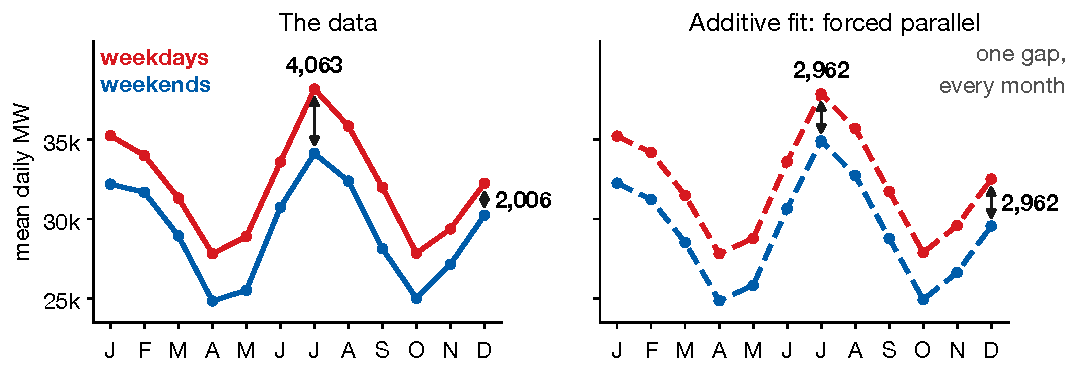
\includegraphics[height=4.3cm]{../Figures/Lecture03_GAMs/additivity_gap.pdf}
  \end{center}
  \vspace{-0.3cm}
  {\small An additive model, month $+$ weekend, can only draw parallel curves: one weekend effect
  for every month. The real gap is twice as big in July as in December. Parallel is the price, and
  also the gift: each effect becomes one curve you can hand to a stakeholder.}
\end{frame}

% =============================================================================
\section{GAM Structure and Smoothing}
% =============================================================================

\sectionslide{GAM Structure and Smoothing}{%
  Additive nonlinear functions, penalized for wiggliness.}

% --- Slide: GAM definition ---------------------------------------------------
\begin{frame}{What Is a GAM?}
  \begin{definitionbox}{Generalized Additive Model}
    \vspace{-4pt}
    \[
      y = \alpha + f_1(x_1) + f_2(x_2) + \cdots + f_k(x_k) + \varepsilon
    \]
    \vspace{-6pt}
    \small where each $f_j(\cdot)$ is a \textbf{smooth, nonlinear function} estimated from
    the data \parencite{Wood2017}.
  \end{definitionbox}
  Each $f_j$ is free to be linear, curved, U-shaped, or threshold-like --- the data decides.
  Because the terms are \emph{added}, each one can be plotted on its own. A smoothness
  penalty, two slides on, keeps them from chasing noise.

  \vspace{0.2cm}
  \textbf{A retail example.} Weekly sales as $f_1(\text{time})$ for the trend, plus
  $f_2(\text{week of year})$ for seasonality, plus $f_3(\text{unemployment})$ for economic
  sensitivity: three curves, each read on its own.
\end{frame}

% --- Slide: what the "Generalized" means -------------------------------------
\begin{frame}{What the ``Generalized'' Actually Means}
  So far every $y$ we have modelled has been continuous and roughly symmetric --- sales in
  dollars, demand in units. For that case an \emph{additive} model is enough.
  The \textbf{G} in GAM is what happens when $y$ is not that kind of variable.
  \begin{definitionbox}{Generalized Additive Model, in full}
    \vspace{-4pt}
    \[
      g\big(\E[y]\big) = \alpha + f_1(x_1) + \cdots + f_k(x_k)
    \]
    \vspace{-6pt}
    \small The additive predictor models a \emph{transformation} of the mean. That
    transformation $g(\cdot)$ is the \textbf{link function}.
  \end{definitionbox}
  \begin{center}
    {\small
    \begin{tabular}{lll}
      \toprule
      \textbf{If $y$ is\ldots} & \textbf{Distribution} & \textbf{Link $g(\cdot)$} \\
      \midrule
      Continuous, symmetric (sales) & Gaussian  & Identity --- $g(\mu)=\mu$ \\
      A count (units, visits, claims) & Poisson   & Log --- keeps the forecast positive \\
      Binary (churn, stockout, yes/no) & Binomial  & Logit --- keeps it inside $[0,1]$ \\
      \bottomrule
    \end{tabular}
    }
  \end{center}
  \vspace{-0.1cm}
  \muted{\footnotesize In \texttt{pyGAM} this is the difference between
  \texttt{LinearGAM}, \texttt{PoissonGAM}, and \texttt{LogisticGAM} --- same additive
  structure, different link. Everything else in this lecture is unchanged.}
\end{frame}

% --- Slide: Smoothness penalty -----------------------------------------------
% Figure: scripts/figures/lecture03_figures.py (smoothing_penalty). basis="ps", not the lab's
% cyclic "cp": with a cyclic basis the lambda -> infinity limit is a flat line, not OLS.
\begin{frame}{Controlling Smoothness: The Penalty Term}
  A GAM minimizes a \textbf{penalized} sum of squared errors:
  \vspace{-0.2cm}
  \[
    \text{PSSE} = \underbrace{\sum_{i=1}^{n}(y_i - \hat{y}_i)^2}_{\text{fit}} +
                  \underbrace{\lambda \int (f''(x))^2\,dx}_{\text{smoothness penalty}}
  \]
  \vspace{-0.45cm}
  \begin{center}
    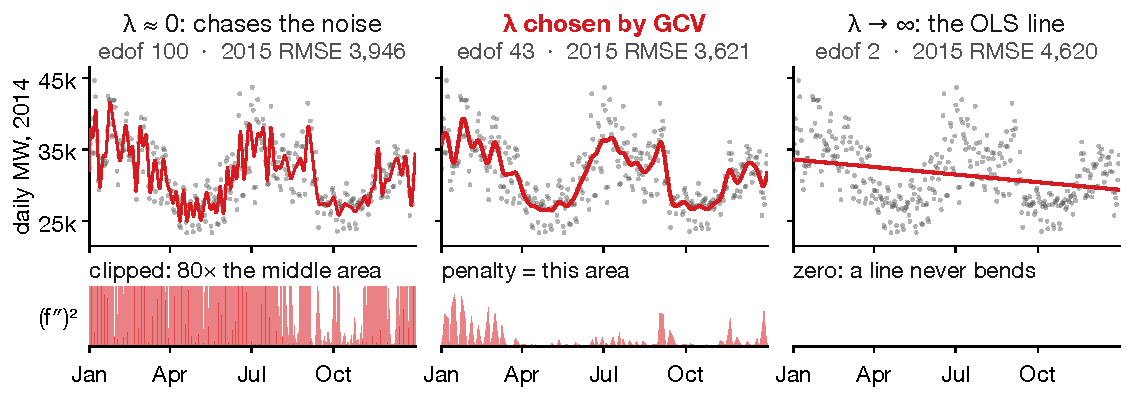
\includegraphics[height=4.0cm]{../Figures/Lecture03_GAMs/smoothing_penalty.pdf}
  \end{center}
  \vspace{-0.35cm}
  {\small $f''$ measures bending, so the penalty is the shaded area: zero only for a straight
  line. Same data, same 100 splines (cubic pieces joined at knots); only $\lambda$ changes,
  and GCV chooses it, not your eye.}
\end{frame}

% =============================================================================
\section{Prophet for Time Series GAMs}
% =============================================================================

\sectionslide{Prophet for Time Series GAMs}{%
  Facebook's Prophet decomposes a time series into trend, seasonality,
  and holiday effects using a GAM.}

% --- Slide: Prophet overview -------------------------------------------------
\begin{frame}{Prophet: Forecasting at Scale}
  \textcite{TaylorLetham2018} built Prophet for large-scale forecasting at Meta. It is a GAM
  in time-series clothing --- the series is decomposed additively:
  \[
    y(t) = \underbrace{g(t)}_{\text{trend}} + \underbrace{s(t)}_{\text{seasonality}}
          + \underbrace{h(t)}_{\text{holidays}} + \varepsilon_t
  \]
  \textbf{Trend $g(t)$}: piecewise linear or logistic, with \emph{changepoints} where the
  slope may shift. \textbf{Seasonality $s(t)$}: a sum of sine waves (a Fourier series), so weekly
  and yearly cycles fit at once. \textbf{Holidays $h(t)$}: irregular events you supply ---
  Black Friday, a launch, a lockdown.

  \vspace{0.2cm}
  Built for analysts, not statisticians: one fit-and-forecast call, robust to gaps and
  outliers, and every component plots on its own.
\end{frame}

% --- Slide: Prophet seasonality, drawn -------------------------------------
% Figure: scripts/figures/lecture03_figures.py (fourier_order) -- Lab 3 Step 2's own fit:
% in-sample RMSE 3,428 MW with one Fourier pair, 1,348 with two (measured.json, "fourier").
\begin{frame}{Prophet's Seasonality: How Many Waves?}
  $s(t)$ is a sum of sine waves. Lab 3's average load for each day of the year, fitted with one
  wave and then with two:
  \begin{center}
    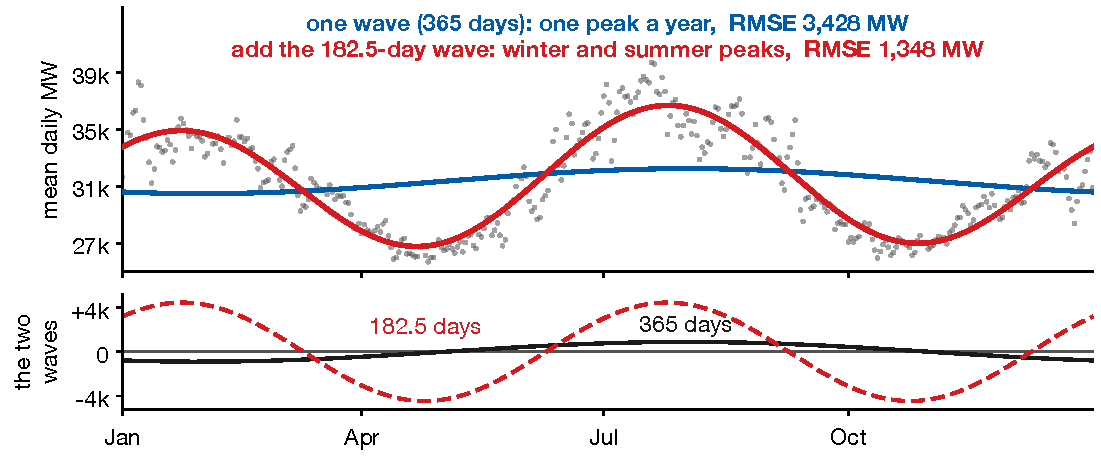
\includegraphics[height=4.6cm]{../Figures/Lecture03_GAMs/fourier_order.pdf}
  \end{center}
  \vspace{-0.3cm}
  {\small A 365-day wave has one peak a year. Heating in January and cooling in July need the
  182.5-day wave too, and adding it cuts the error by a factor of 2.5. Prophet's yearly term uses
  10 such pairs by default.}
\end{frame}

% --- Slide: Prophet code -----------------------------------------------------
% Figure: scripts/figures/lecture03_figures.py (prophet_components) -- Lab 3 Step 3's own fit,
% trained 2013 to July 2017; the shaded strip is the lab's test year.
\begin{frame}{Prophet: Code and Workflow}
  \begin{examplebox}{Prophet on Lab 3's Electricity Data}
    {\scriptsize
    \texttt{from prophet import Prophet}\\
    \texttt{m = Prophet(yearly\_seasonality=True, weekly\_seasonality=True, daily\_seasonality=False)}\\
    \texttt{m.fit(train)\ \ \ \ \# a DataFrame with columns ds and y}\\
    \texttt{fc = m.predict(test);\ \ m.plot\_components(fc)}
    }
  \end{examplebox}
  \vspace{-0.25cm}
  \begin{center}
    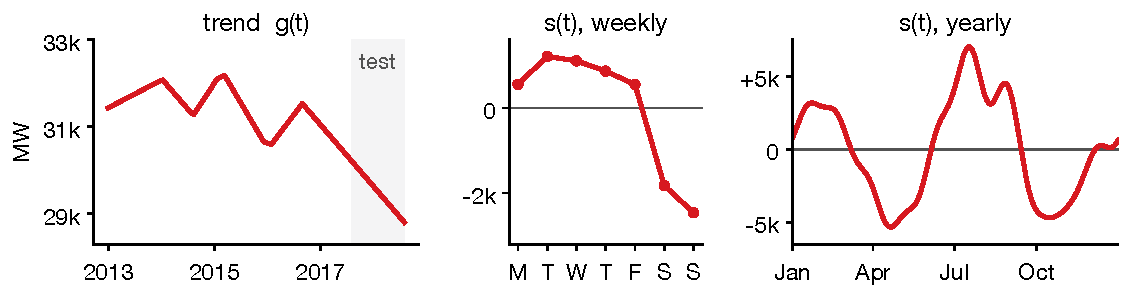
\includegraphics[height=3.1cm]{../Figures/Lecture03_GAMs/prophet_components.pdf}
  \end{center}
  \vspace{-0.35cm}
  {\small \texttt{plot\_components} draws one panel per additive term. \textbf{Reach for
  Prophet} when someone will ask you to explain the forecast; \textbf{reach for pyGAM} when you
  have many correlated external predictors.}
\end{frame}

% =============================================================================
\section{pyGAM for General Additive Modeling}
% =============================================================================

\sectionslide{pyGAM for General Additive Modeling}{%
  When you have multiple predictors and want flexible nonlinear effects
  for each.}

% --- Slide: pyGAM overview ---------------------------------------------------
\begin{frame}{pyGAM: Flexible Additive Modeling}
  \texttt{pyGAM} fits a GAM with a smooth function you specify per predictor:
  \begin{examplebox}{pyGAM Example}
    {\footnotesize
    \texttt{from pygam import LinearGAM, s, f, l}\\[2pt]
    \texttt{gam = LinearGAM(s(0) + s(1) + s(2) + f(3))}\\
    \texttt{gam = gam.gridsearch(X, y)}\\[2pt]
    \texttt{pdep, confi = gam.partial\_dependence(term=0, width=0.95)}\\
    \texttt{y\_hat = gam.predict(X\_new)}
    }
  \end{examplebox}
  The three term types are the whole vocabulary: \texttt{s(j)} is a smooth spline of
  feature $j$ --- the flexible nonlinear effect; \texttt{l(j)} forces a straight line, which
  is worth using when theory says the effect should be linear; and \texttt{f(j)} handles a
  binary or categorical feature.

  \vspace{0.15cm}
  \texttt{gridsearch} then tunes $\lambda$ by cross-validation --- though you should still
  look at the resulting curves and ask whether they are plausible.
\end{frame}

% --- Slide: Partial dependence -----------------------------------------------
% Figure: scripts/figures/lecture03_figures.py (partial_dependence) -- Lab 3's own model,
% s(doy, cyclic) + f(dow), fitted on 2013 to July 2017.
\begin{frame}{Interpreting GAM Results: Partial Dependence Plots}
  Each panel is one $\hat{f}_j(x_j)$ with its confidence band, from Lab 3's electricity model:
  \begin{center}
    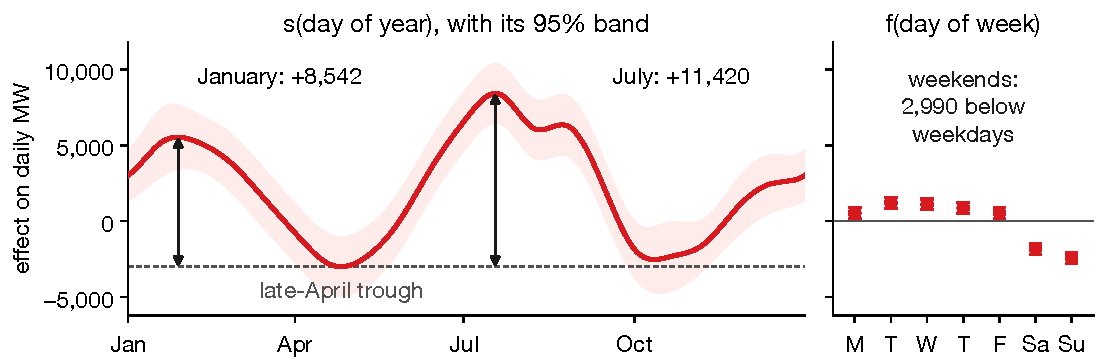
\includegraphics[height=3.5cm]{../Figures/Lecture03_GAMs/partial_dependence.pdf}
  \end{center}
  \vspace{-0.35cm}
  {\small Read the band too. Every day of the year is equally covered, so it barely changes
  width; where data thin out it fans, just where readers want to extrapolate.}
  \begin{keybox}
    \small A sentence someone can act on: \emph{``plan for mid-July demand about 11,400 MW
    above the late-April trough, a winter peak about 8,500 above it, and weekends about 3,000
    below weekdays.''} No straight line in day of year has two peaks.
  \end{keybox}
\end{frame}

% =============================================================================
\section{Key Takeaways and Roadmap}
% =============================================================================

\sectionslide{Key Takeaways and Roadmap}{%
  GAMs: flexible, interpretable, and underutilized in business forecasting.}

% --- Slide: GAMs vs. alternatives --------------------------------------------
\begin{frame}{GAMs vs.\ Other Methods: When to Choose Each}
  \begin{center}
    {\small
    \begin{tabular}{lllll}
      \toprule
      \textbf{Method} & \textbf{Nonlinear} & \textbf{Interactions} & \textbf{Interpretable} & \textbf{Use case} \\
      \midrule
      ARIMA / ETS       & No  & No     & High   & Univariate time series \\
      Linear regression & No  & Manual & High   & Few predictors \\
      \textbf{GAM}      & Yes & No     & High   & Few predictors, explain effects \\
      Random Forest     & Yes & Yes    & Medium & Many predictors, tabular \\
      XGBoost           & Yes & Yes    & Low    & Many predictors, accuracy first \\
      \bottomrule
    \end{tabular}
    }
  \end{center}

  \vspace{0.15cm}
  The column that decides it is usually \textbf{Interactions}. A GAM is additive by
  construction, so if the effect of price depends on whether it is a holiday week, a GAM
  cannot represent that and a tree can.

  \vspace{0.15cm}
  \textbf{Choose a GAM when} you must explain each predictor's effect, the effects are curved,
  or a series has complex trend and seasonality (Prophet), and interpretability matters more
  than the last few points of accuracy. Whether a flexible model buys those points is an
  empirical question; Lectures 4--6 test it.
\end{frame}

% --- Slide: Key takeaways ---------------------------------------------------
\begin{frame}{Lecture 3: Key Takeaways}
  \begin{keybox}
    {\small
    \begin{enumerate}
      \item \textbf{GAMs}, $y = \alpha + f_1(x_1) + \cdots + f_k(x_k) + \varepsilon$: nonlinear,
            yet additive, so each effect plots on its own.
      \item The \textbf{smoothness penalty} prices bending; $\lambda$, chosen by GCV or
            cross-validation, trades fit against smoothness.
      \item \textbf{Prophet} is a GAM for time series: trend + seasonality + holidays.
      \item \textbf{pyGAM}: \texttt{s()} smooth, \texttt{l()} linear, \texttt{f()} categorical;
            \texttt{gridsearch} tunes $\lambda$.
      \item \textbf{Partial dependence plots} turn the model into sentences a stakeholder can
            act on.
    \end{enumerate}
    }
  \end{keybox}
  \muted{\itshape Next: Decision Trees --- moving to tree-based methods
  that capture interactions automatically.}
\end{frame}

% --- References ---------------------------------------------------------------
\begin{frame}[allowframebreaks]{References}
  \printbibliography[heading=none]
\end{frame}

% =============================================================================
\end{document}
% =============================================================================
